\documentclass[12pt, a4papre]{article}
\usepackage[catalan]{babel}
\usepackage[unicode]{hyperref}
\usepackage{amsmath}
\usepackage{amssymb}
\usepackage{amsthm}
\usepackage{xifthen}
\usepackage{listings}
\usepackage{float}
\usepackage{siunitx}
\usepackage{graphicx}
\usepackage{indentfirst}

\newcommand{\norm}[1]{\lvert #1 \rvert}
\graphicspath{ {./Images/} }

\hypersetup{
    colorlinks = true,
    linkcolor = blue
}

\author{Elexioma de l'acció}
\title{31. A l'aventura}
\date{}

\begin{document}
	\maketitle
	
	En aquest cas li haurem de donar gracies a la ma dreta que ens atura de construir un mon sota fonaments enginyerils. Aquí li portem un paio a l'Enric per a que se senti satisfet.
	
	\begin{proof} Definim la funció contraexemple $f(x, y)$ de la següent forma:
	
	\[
	f(x, y)= \left\{ \begin{array}{lccc}
			0 &   si  & y \geq x^2  & y \leq 3x^2 \\
			\\ y-3x^2 &  si & 2x^2 \leq y \leq 3x^2 \\
			\\ x^2-y &  si  & x^2 \leq y \leq 2x^2 
			\end{array}
	\right.
	\]
	
	\begin{figure}[H]
		\begin{center}
		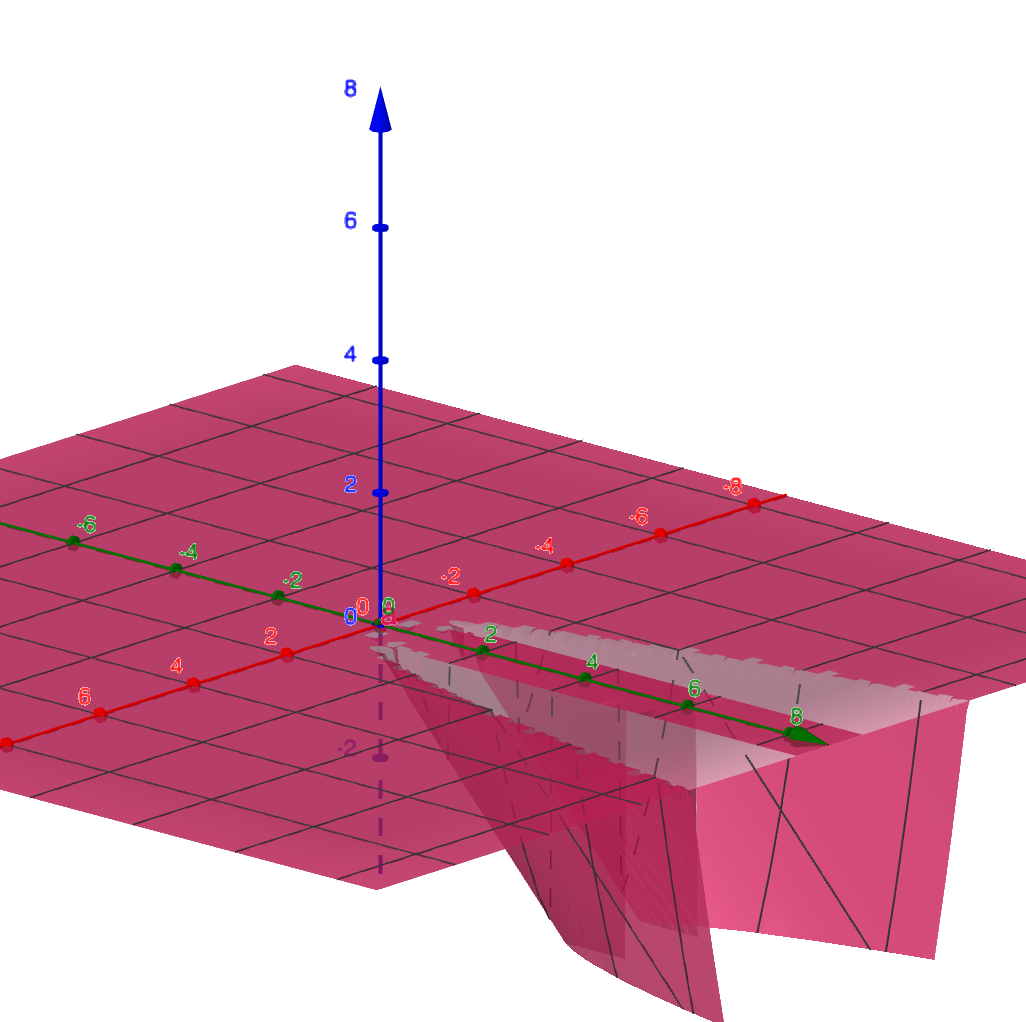
\includegraphics[width=75mm]{graph1.png}
		\caption{Grafica de la funció en cuestió}
		\end{center}
	\end{figure}
	
	Aquesta funció es continua ja que pel lema d'enganxament, cada funció es continua al seu tros i a la intersecció coincideixen:
	
	\[
		f(x, 2x^2) = 2x^2-3x^2=x^2-2x^2=-x^2 \qquad f(x, x^2) = x^2-x^2 = 0 
	\]
	\[
		 f(x, 3x^2) = 3x^2 - 3x^2 = 0
	\]
	
	Veiem primer que el punt $(0, 0)$ no es mínim. Considerem la restricció de la funció a la paravola $y=2x^2$. Aleshores tenim que 
	
	\[
		f|_{y=x^2} = -2x^2 \implies (f|_{y=x^2})' = -4x \implies (f|_{y=x^2})'' = -4
	\]
	
	Per tant restringint la funció a aquest cami veiem que te un maxim al origen.
	
	Veiem ara que la funció restringida a cualsevol recta te un minim local al origen. Cualsevol recta que passi per l'origen a part de la recta $y=0$ i $x=0$ tallarà la parabola $3x^2$ 2 cops, un d'ells al origen i l'altre al punt $(k, 3k^2)$ suposant que la recta es $kx=y$.
	
	Per tant si considerem la bola $B_{\frac{min(k, 3k^2)}{2}}(0, 0)$ la recta $y = kx$ només tallarà amb la paràbola al origen i a mes es cumplirà per tot punt de la recta $y \geq 3x^2 \implies f(x, kx) = 0$ i per tant la restricció de la funció a la recta te un minim local al origen, al ser aquesta constant dins de la bola. Els casos de recta $y=0$ i $x=0$ son trivials.
	
	
	\end{proof}
	
	
	
	
\end{document}